\documentclass[draft]{article}

% if you need to pass options to natbib, use, e.g.:
% \PassOptionsToPackage{numbers, compress}{natbib}
% before loading nips_2016
%
% to avoid loading the natbib package, add option nonatbib:
% \usepackage[nonatbib]{nips_2016}

\usepackage{nips_2016}

% to compile a camera-ready version, add the [final] option, e.g.:
% \usepackage[final]{nips_2016}

\usepackage[utf8]{inputenc} % allow utf-8 input
\usepackage[T1]{fontenc}    % use 8-bit T1 fonts
\usepackage{hyperref}       % hyperlinks
\usepackage{url}            % simple URL typesetting
\usepackage{booktabs}       % professional-quality tables
\usepackage{amsfonts}       % blackboard math symbols
\usepackage{nicefrac}       % compact symbols for 1/2, etc.
\usepackage{microtype}      % microtypography

\usepackage{graphicx}  % Required for including images


\title{Formatting instructions for NIPS 2016}

% The \author macro works with any number of authors. There are two
% commands used to separate the names and addresses of multiple
% authors: \And and \AND.
%
% Using \And between authors leaves it to LaTeX to determine where to
% break the lines. Using \AND forces a line break at that point. So,
% if LaTeX puts 3 of 4 authors names on the first line, and the last
% on the second line, try using \AND instead of \And before the third
% author name.

\author{
  David S.~Hippocampus\thanks{Use footnote for providing further
    information about author (webpage, alternative
    address)---\emph{not} for acknowledging funding agencies.} \\
  Department of Computer Science\\
  Cranberry-Lemon University\\
  Pittsburgh, PA 15213 \\
  \texttt{hippo@cs.cranberry-lemon.edu} \\
  %% examples of more authors
  %% \And
  %% Coauthor \\
  %% Affiliation \\
  %% Address \\
  %% \texttt{email} \\
  %% \AND
  %% Coauthor \\
  %% Affiliation \\
  %% Address \\
  %% \texttt{email} \\
  %% \And
  %% Coauthor \\
  %% Affiliation \\
  %% Address \\
  %% \texttt{email} \\
  %% \And
  %% Coauthor \\
  %% Affiliation \\
  %% Address \\
  %% \texttt{email} \\
}

\begin{document}
% \nipsfinalcopy is no longer used

\maketitle

\begin{abstract}
  We are comparing the effect of pretraining.
\end{abstract}

\section{Introduction}
\section{Related Work}
\section{Setup \& Context}
  \subsection{General Setup}
    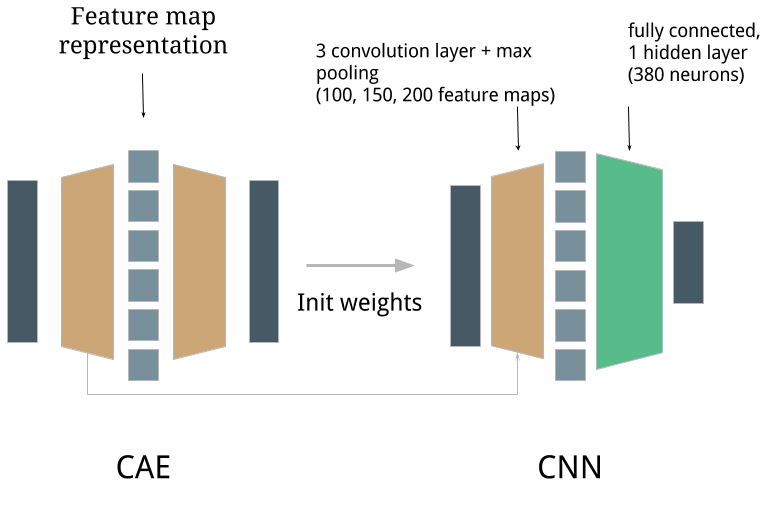
\includegraphics[width=0.8\linewidth]{../graphics/setup.png}
  \subsection{Autoencoder Training}

  \subsection{Pre-Training and Test Methodology}
  

\section{Experiments}

  \subsection{Datset Descriptions and Challenges}

    \begin{itemize}
    \item{MNIST}
        MNIST is the standard dataset used for image classification. It consists of scanned postal code numbers (?),
        which are 28 by 28 pixel grayscale images.
    \item{CIFAR-10}
        The CIFAR dataset is made out of natural scenes, which are 32x32 colorized images. The CIFAR-10 variant,
        which we used, is built as a classification dataset with 10 specified labels (cars, cats...)
    \item{CK+}
        The Extended Cohn-Kanade (CK+) dataset was the most interesting dataset during our project. Unlike the other
        two datasets, no pre-training experiments have been done on CK+, as far as we know.
        As the CK+ is not readily prepared for running those kinds of experiments, we had to put some work into this ourselves.
        We decided to not take the full images, but to use the provided facial landmarks, to put the faces
        into a bounding box of size (...).
         
    \end{itemize}

  \subsection{Autoencoder Training}
  For the autoencoder training we took each of the three datasets' images, reshaped them into a vector and used
  these values as input and target output for a convolutional autoencoder.
  \subsection{Pretraining and Classification}
  The general idea of pretraining a classification neural network, is to transfer the encoding weights of
  the CAE to the CNN. So we took the convolutional filter weights, which we generated during the autoencoder training,
  and used them as initial values for the convolutional layers for the classification network.

  As the MNIST and CIFAR-10 datasets consist of a lot more images than CK+, we decided to follow the approach of the paper
  and take a 1k and 10k subset for these two. So while we still took all training images for building a decent autoencoder,
  the CNN could only use some of the images. This is especially interesting to check the hypothesis, that pre-training makes
  more sense, when you have less training images.

  To validate our pretraining experiments, in each run we set up a CNN with randomly initialized filters and a CNN which
  uses the filters trained by the CAE. Both networks have randomly initialized weights for their dense layers.


\section{Discussion and Conclusion}
  
  \begin{itemize}

    \item Evaluation of the Results         (Does it work)
    \item Evaluation of further experiments (When does it work, comparison with relu etc)

  \end{itemize}

\end{document}
